\chapter{Prototype Solution}
\label{chapter:prototype}

In Section \ref{sec:benchmarking} existing solutions for the problems of
publishing, sharing and managing research data are presented. It is clear that
since these solutions exist, there is no point in reinventing the wheel and
implement a new system. Instead we have implemented a local installation
of some of the systems presented in the benchmarking section. From the test
installations we have chosen the one that works the best and used that to
run tests on potential users of the system. The tests are used to gain insights
on what the finalized system should look like. It is also notable
that the existing solutions are remarkably similar as noted in as noted
in Section \ref{sec:benchmarking}, so using any one of them
would give applicable results.

The prototype solution focuses on publishing and sharing of research data. The
other option would have been to focus on the research data management during
the research project, but research projects last longer than the span of this
thesis and the results gained from that avenue of research that would likely be quite superficial.
The lack of culture and practices are a factor for both publishing and
and managing research data. The lacking of research data management culture is
due to the lack of education and need for it, whereas publishing research data
is a moderately new phenomenon and the culture is still being formed. This makes it a more novel subject
of study. Increased demand for research data sharing and publishing would also
force research data management practices to be developed further.

We ended up choosing the Harvard Dataverse solution to be the prototype for our
purposes. The following sections detail the rationale behind this choice, the
technical details of the system and the tests that were conducted using the
system along with the learnings.

\section{Rationale behind selecting Dataverse}

As a part of the benchmarking the existing solutions and in order to select the
right tool to run tests on users we tried installations of a Hydra head (Hydra head is a
Hydra instance in the Hydra Project terminology), a
Zenodo instance and a Harvard Dataverse instance. These three were chosen
because they represent different technologies and are widely adopted as tools
for publishing research data.

Setting up a Hydra head is fairly simple using Ruby
Gems\footnote{\url{https://github.com/projecthydra/hydra-head}}.
Setting up the basic Hydra head
does not get you far, however, since after setting up the installation you need
to define your data model and almost everything else on your repository.

This setup cost makes Hydra a very versatile framework. It is being used on many
places beyond just research institutions, such as museums and image
repositories\footnote{\url{https://wiki.duraspace.org/display/hydra/Partners+and+Implementations}}.
Many of these systems are built on Hydra solution
bundles\footnote{\url{https://wiki.duraspace.org/display/hydra/Hydra+Solution+Bundles}}
which are also
are open source. Installations of a clean Hydra head and the version
run by Penn State University\footnote{\url{https://scholarsphere.psu.edu/}} were tried.

The conclusion about Hydra heads was that while the system is modern and quite
easy to install, the setup of the system made it too time consuming to setup a
testing prototype in a reasonable time frame. The system is flexible and if you
wanted to build your own customized repository solution Hydra would be suitable
for that. The Penn State implementation was heavily branded and tweaked for
their purposes, making it hard to make it work for prototyping purposes.
Blacklight\footnote{\url{http://projectblacklight.org/}},
the frontend library used by the Hydra
project, is quite good and makes for easy to use and efficient frontends.

We tried installing Zenodo system locally from the source
code\footnote{\url{https://github.com/zenodo/zenodo}}, but could not get the
build process to work correctly as of writing of this thesis.
It was later found out that the Zenodo system, which is built upon the Invenio
archiving software, is notoriously hard to install according to the people who
originally built it\footnote{M. Nurmela and D. Lecarpentier, personal
communication, September 30th, 2015}.

Due to the problems with the installation the Zenodo system was ruled out at
the prototyping phase.

Harvard Dataverse is easy to install with the installation instructions as
both a development version from the source
code\footnote{\url{http://guides.dataverse.org/en/latest/developers/index.html}} and a
production version with
the installation bundle\footnote{\url{http://guides.dataverse.org/en/latest/installation/}}.

The easy installation immediately gave a functioning software repository to
conduct tests with and that lead to the decision to use Dataverse as the
prototype to test current data repository solutions and gain user feedback to
supplement the other research.

Though implemented in different technologies, the functioning of the existing
research data repository systems is quite similar. All of them offer form based
dataset uploads, full text searches and some forms of access control. Many of
them are even built on same technologies, such as Solr indexing
software\footnote{\label{solr}\url{http://lucene.apache.org/solr/}} or
postgreSQL\footnote{\label{postgre}\url{http://www.postgresql.org/}}.

The similarity of the systems as well as the fact that there is no global
consensus on what repository software is the best in business hints that you
could use any one of them in your organization. From this angle it also makes
sense to use one of them to gain user insights and figure out how the systems
should be developed in order to satisfy the user needs better.

\section{Users of the system}
\label{sec:users}

As examined in Section \ref{chapter:positioning}, a research data repository
systems have many stakeholders. Identified key stakeholders are presented in
the following:

\begin{itemize}
    \item Researchers,
    \item University courses,
    \item Research groups,
    \item Librarians,
    \item Students,
    \item IT staff; and
    \item Other interested parties.
\end{itemize}

The requirements of these different stakeholders are boiled down to user
stories, which are presented in Appendix \ref{chapter:first-appendix}.

\section{Prototype system description}
\label{sec:system_description}

Harvard Dataverse is a Java application. Other technologies employed are Apache
Solr\footnotemark[\getrefnumber{solr}] for indexing the database to facilitate search,
postgreSQL\footnotemark[\getrefnumber{postgre}] for database
and Glassfish or Apache for serving the
web pages\footnote{\url{https://glassfish.java.net/}, \url{https://httpd.apache.org/}}.
Dataverse also has in built support for the R statistical computing
language\footnote{\url{https://www.r-project.org/}} for running simple
statistical analyses on the data and for data visualization using the
TwoRavens tool \cite{DBLP:conf/ht/HonakerD14}.

The class model of
Dataverse\footnote{\label{architecture}\url{https://github.com/IQSS/dataverse/tree/4.3/doc/Architecture}}
is described in Figure \ref{fig:dataverse-model}.

\begin{figure}
    \begin{centering}
        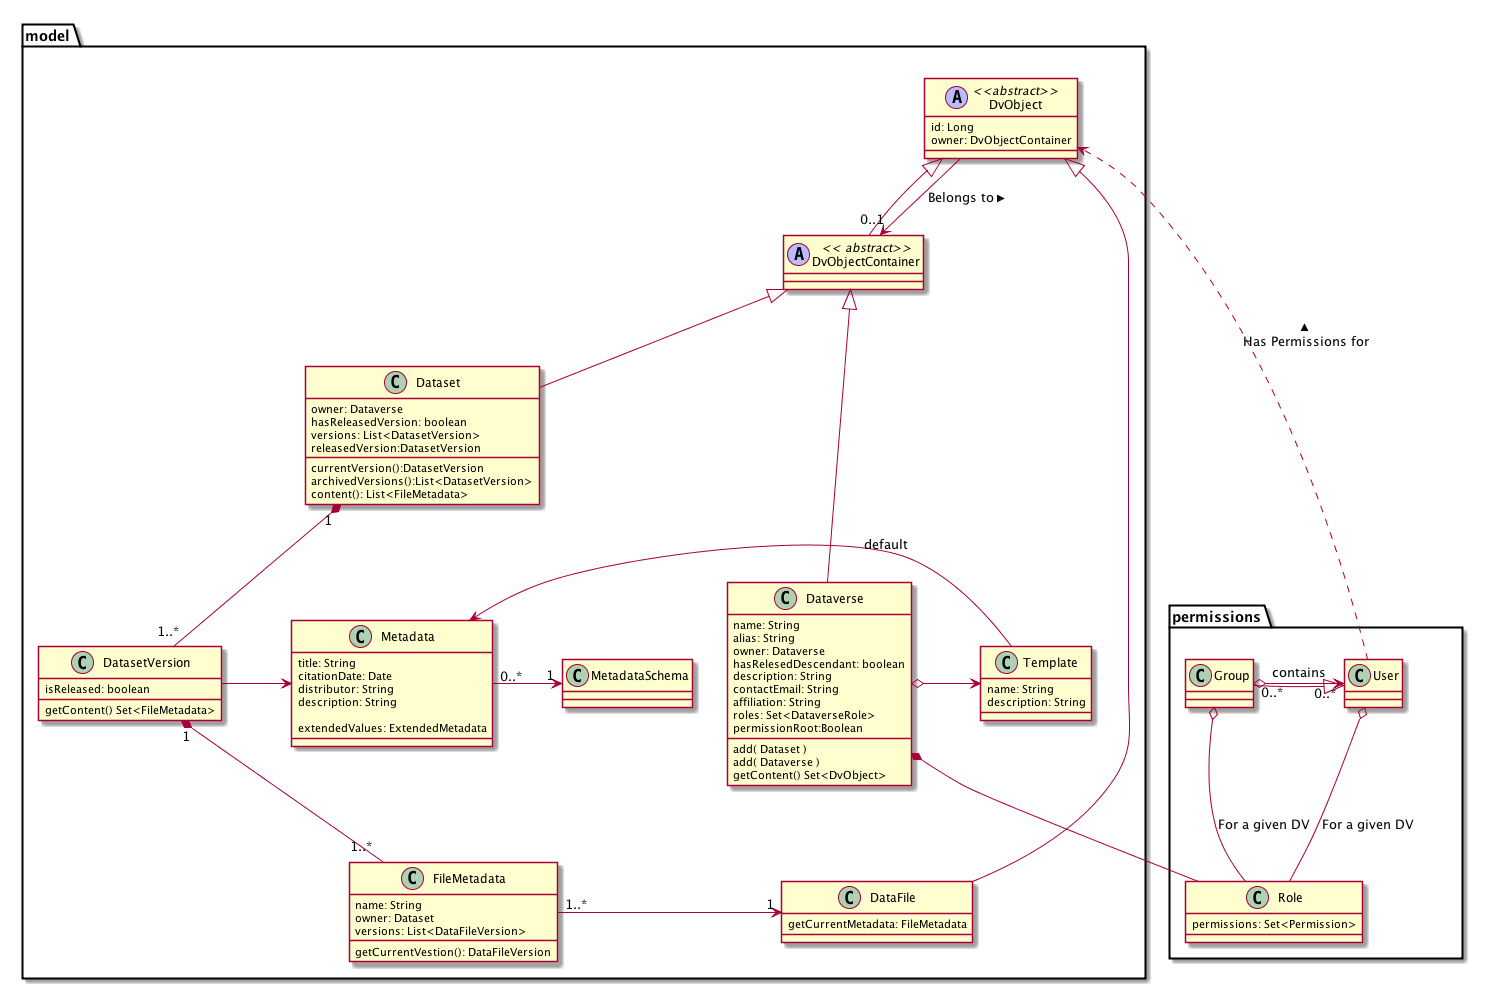
\includegraphics[width=\textwidth]{images/dataverse-model}
    \end{centering}
    \caption[The Dataverse class model]{The Dataverse class model\footnotemark[\getrefnumber{architecture}]}
    \label{fig:dataverse-model}
\end{figure}

In the heart of Dataverse is the division of content into Dataverses. The
closest analogue to a Dataverse is a normal folder in a typical file system -
Dataverses can contain other Dataverses, but in the place of files Dataverses
contain datasets. Datasets, in turn, contain the files that make up the
dataset. The Dataverse split of the system also allows for fine grained access
control, since Dataverses can be shared with no one, with single users or user
groups.

Users can use the Dataverse
with either the web user interface or the API offered by Dataverse. The
dataflow and interplay of the different components of the Dataverse application\footnotemark[\getrefnumber{architecture}] is shown in Figure
\ref{fig:dataflow}.

\begin{figure}
    \begin{centering}
        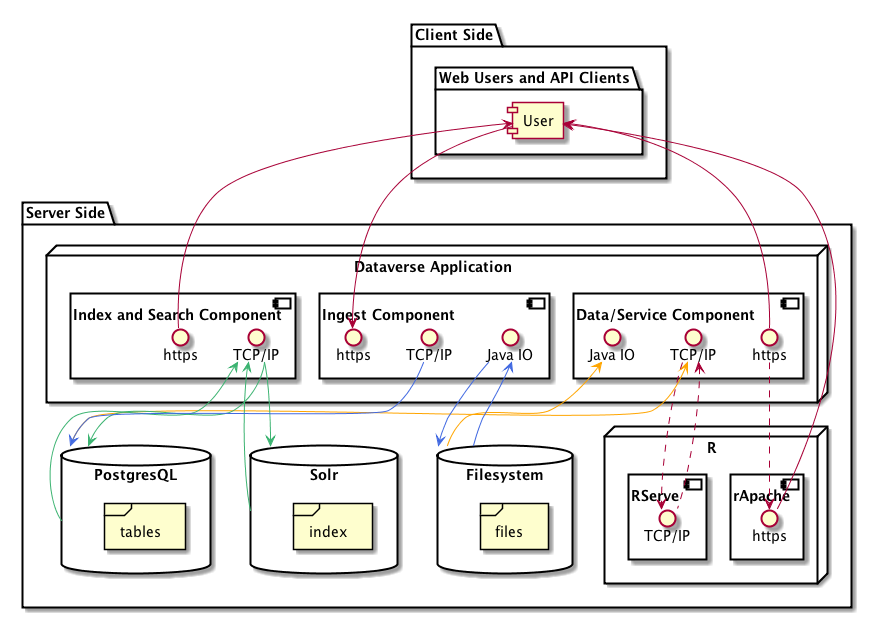
\includegraphics[width=\textwidth]{images/dataflow}
    \end{centering}
    \caption[The Dataverse application dataflow]{The Dataverse application dataflow\footnotemark[\getrefnumber{architecture}]}
    \label{fig:dataflow}
\end{figure}

The Dataverse Java application encompasses the Client Side and Dataverse
Application in Figure \ref{fig:dataflow}. Ingest refers to uploading datasets
to the system and the Index and Search and Data/Service components serve the
user the desired content, be it search results or data to be downloaded. The
rApache component handles the data visualization and runs the TwoRavens tool,
and RServe is used for the statistical computation when the user requests that.

Two versions of the Dataverse system were installed - one from source
code\footnote{\url{https://github.com/quarian/dataverse}} and one from the
installation bundle provided by the developers of
Dataverse\footnote{\url{https://github.com/IQSS/dataverse/releases/tag/v4.2}}.
The installations were run in the CSC cPouta
environment\footnote{\url{https://research.csc.fi/cpouta}}, which is an
OpenStack instance\footnote{\url{https://www.openstack.org/}}. The source code
installation is referenced from now as the development installation. It
was used to get a feel of the code and the system quality and the access
to the source makes debugging weird situations easier.
The installation from the installation bundle is referred to as the production
installation. The installation bundle should provide a more stable system than the branch of development
code that was forked for the development installation. Figure
\ref{fig:cpouta} shows the different installations in the cPouta environment.

\begin{figure}[t]
    \centering
    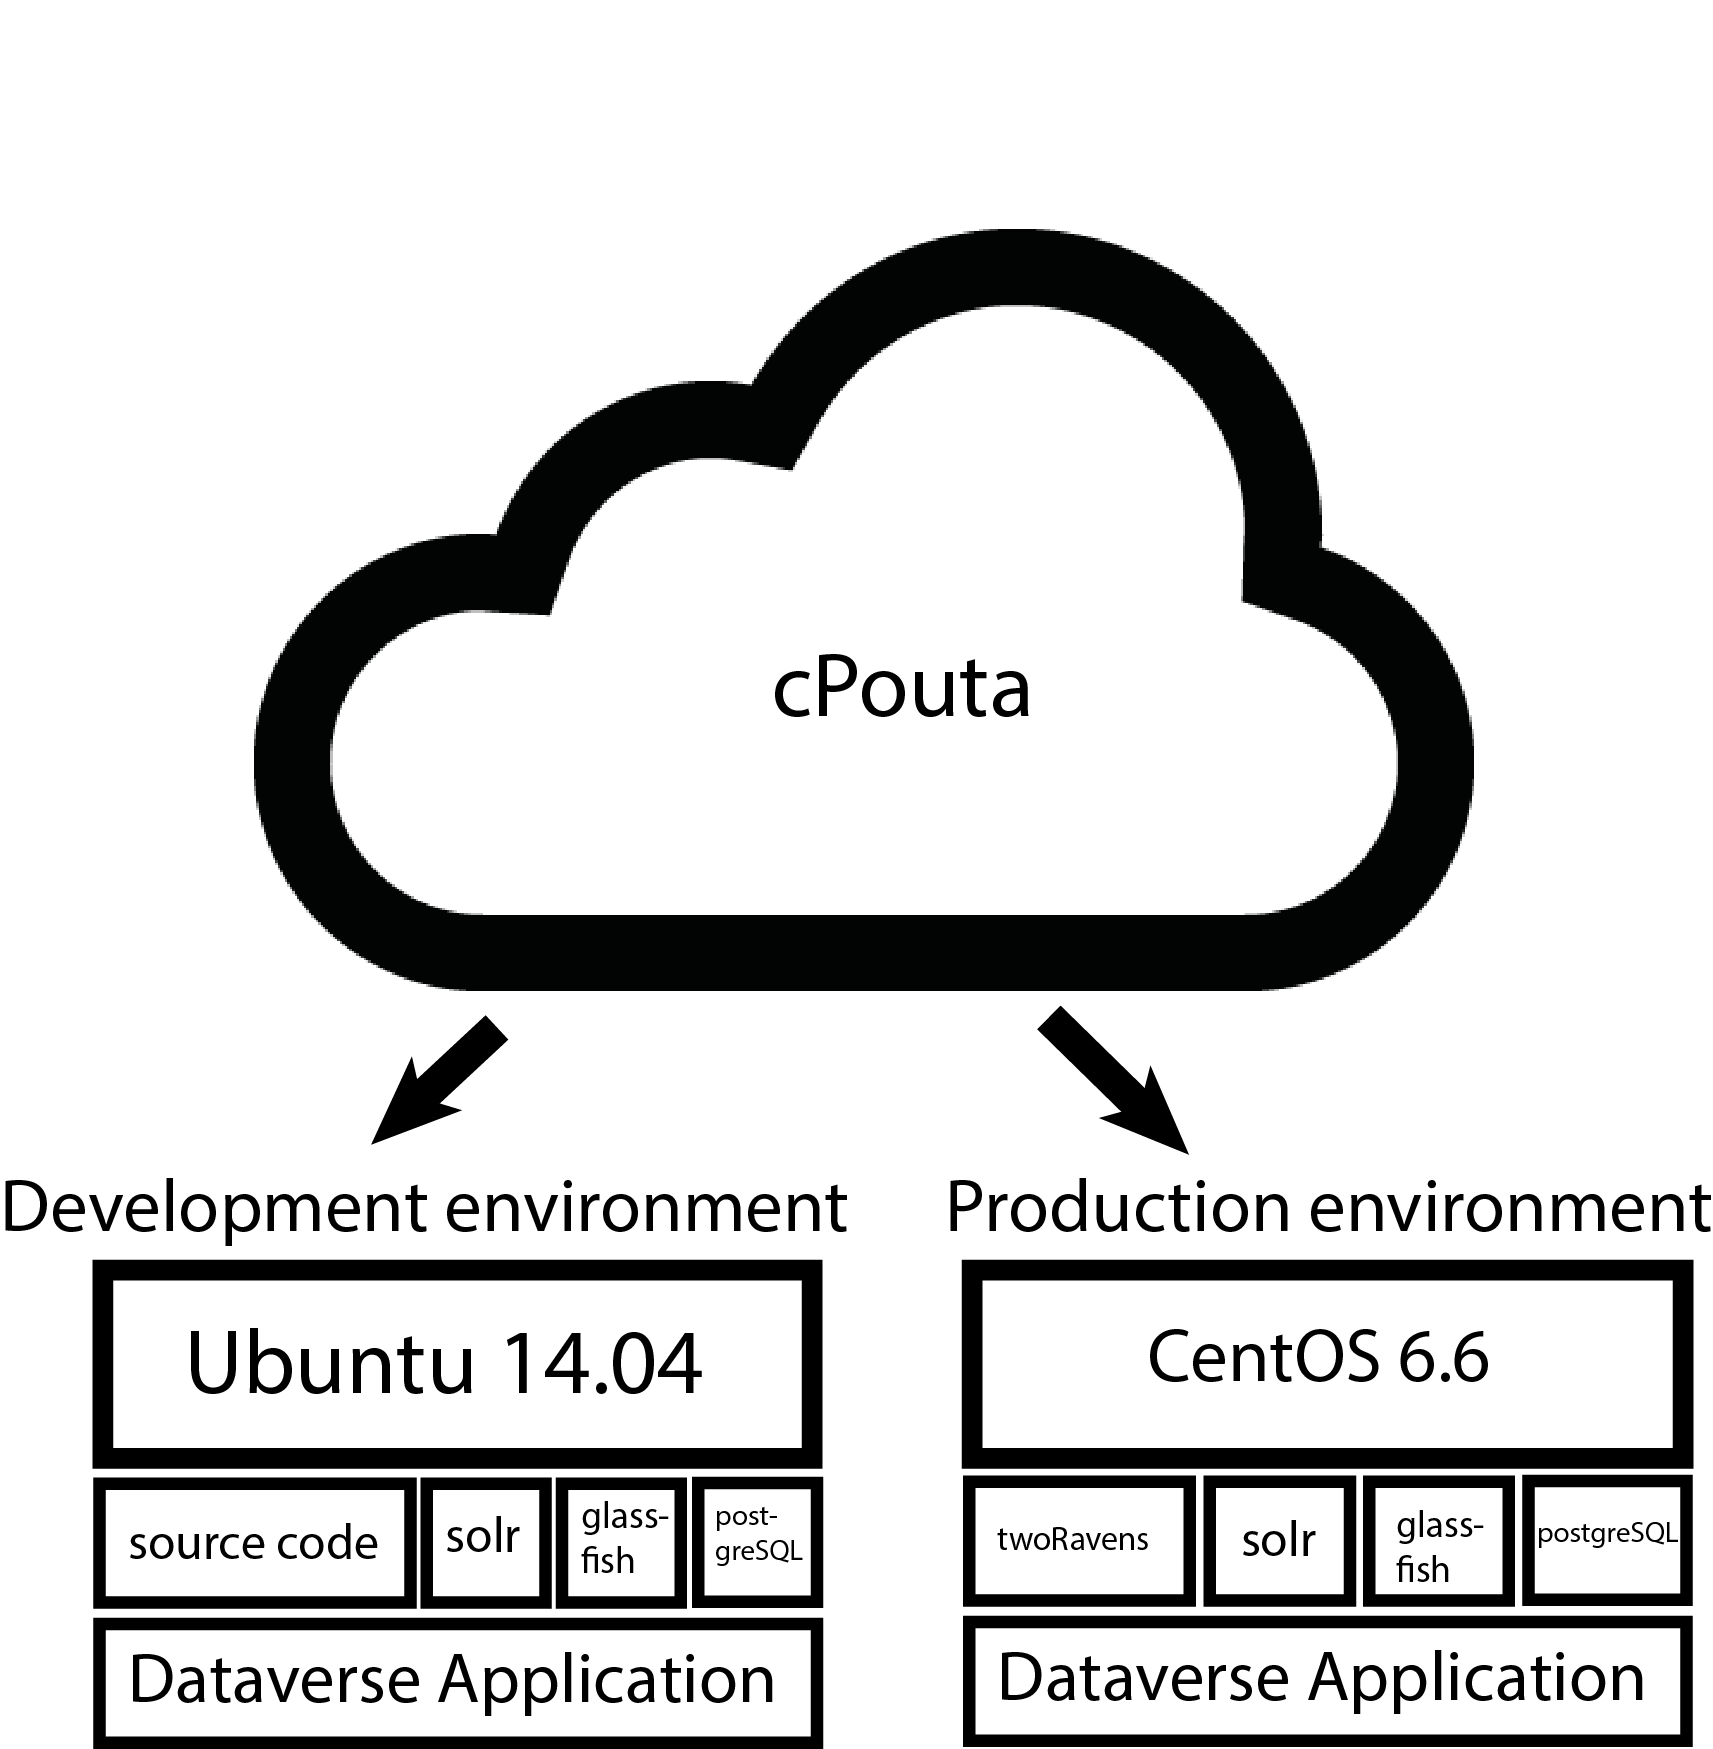
\includegraphics[width=0.7\textwidth]{images/cpouta2}
    \caption{The different installations in the cPouta environment}
    \label{fig:cpouta}
\end{figure}

The development installation is installed on top of Ubuntu 14.04 and it
works, even though the installation instructions propose the use of Red Hat
based systems. The TwoRavens application is omitted from the development
installation, since the data visualization is not the core functionality of
the research data repository software. The production installation is done
on CentOS 6.6, which is a derivative of Red Hat Linux. The installation was
first tried on CentOS 7.0, but the differences between CentOS 6.x and 7.x made
it so that the installation would not work - CentOS 6.6 was settled to be the
final environment of the development installation.

As for the information security of the prototype solution, the development
installation is not set up with any firewall rules or other security, since
its purpose is to get a feel of the system. For the production installation
firewall rules are set using the security groups functions of OpenStack.
Inbound TCP/IP traffic was only allowed to port 8080, which Glassfish was
listening to.
When it comes to research data, security is important, and since the
technologies such as Glassfish and postgreSQL are well known software and
their default passwords and ports are well known setting up firewalls and
changing those passwords is imperative. Additionally, with Dataverse,
firewalling the port that Apache Solr uses is important, since it circumvents
the user credentials and it could be used to retrieve any indexed information
in the system.

To replicate the test systems follow the installation
instructions\footnote{\url{http://guides.dataverse.org/en/latest/installation/}}
and the description here.

\section{System test setup}
\label{sec:system_testing}

In order to extract value from the prototype Dataverse it needed to be tested
with actual users. Of all the stakeholders groups presented in Section \ref{sec:users}
the research scientists is the most important one, since without them there is
no research data and without them using the research data repository there is
no public research data. Section \ref{chapter:positioning} summarizes learnings
from the other stakeholder groups. Section \ref{chapter:positioning} also contains results from
surveys conducted on research data management and sharing to provide context
also from the point of view of researchers.

To test this system we worked together with the Complex Networks
Group\footnote{\url{http://becs.aalto.fi/en/research/complex\_networks/}} and the
Speech Group\footnote{\url{http://research.ics.aalto.fi/speech/}} of Aalto
University. Two kinds of tests were designed and implemented. The first test was a contextual
interview - which means an interview and observation conducted in the user's normal working
environment. The contextual interviews were conducted both with
the development installation of the Dataverse as a tool for discussion and as
conversations and observations about the current state of research data management and the
current working practices. The second test was conducted with two lead users
and the production Dataverse installation. The users were asked to input their
datasets to the Dataverse and fill in the appropriate metadata.

The contextual interviews focused on the current methods of research data
management and sharing. The users were asked to describe their practices and
how they had come across to them (taught by the university, learned on their
own or some other methods). When applicable, the users were asked to show
their current setups for research data management and sharing. When the
development Dataverse was used the users were asked to upload a test dataset
to the Dataverse and walk the interviewer through the thought process. In
addition the interviewees were asked to use the actual Harvard
Dataverse\footnote{\url{https://dataverse.harvard.edu/}} to find datasets
relevant to their field of study and talk through the process. All these
interactions were also observed to find out usability and other issues that
might arise during the exchanges. In total 10 members of the Complex
Networks group were involved in the contextual interviews.

The lead users were granted access to the development Dataverse and were
briefly instructed to the different functionalities of Dataverse. The
instructions were left vague in order to make them read the relevant user
guides and provide feedback on how easy the system was to use after only very
brief instructions. After roughly a month's time the lead users were debriefed
and interviewed about their experiences with the Dataverse system.

The goal of these tests was to understand the current status of research data
management and publishing, how a research data publication system would fit
this status and how well does the research data publication system fill its
designated role. The usability of the system is also a point of interest.

In addition the installation and maintenance of the prototype installations
would give insight on how the system would be to maintain and how it would work
from a technical point of view.

\section{Outcomes of the prototype and the tests}
\label{sec:prototype_outcomes}

The contextual interviews and lead user tests yielded results on technical matters,
user interface and experience matters and on the current status of the research
data management and publishing.

The results of the tests showed that the technical implementations for research
data sharing fill their role. In the contextual interviews it was clear that
the manual uploading and searching worked fine - the users were able to pick up
the process of searching and uploading datasets quickly. The upload process is form
based, shown in Figure \ref{fig:upload} which is similar to many
form based upload pages you can find online. Files for datasets can be dragged and
dropped to the user interface or the file browser of the computer can be used. The users
were able to find the suitable method for them from the two options. But even
though the upload process is mechanically easy, the upload form contained a part
where the user was supposed to insert keywords of the dataset being uploaded.
The keywords come with the concept of vocabulary that was not known to the
users. The point of confusion is shown in Figure \ref{fig:vocabulary}. In this context vocabulary
refers to a set of words that have been agreed upon within a field of science
in order to standardize communication within the field.

\begin{figure}
    \begin{centering}
        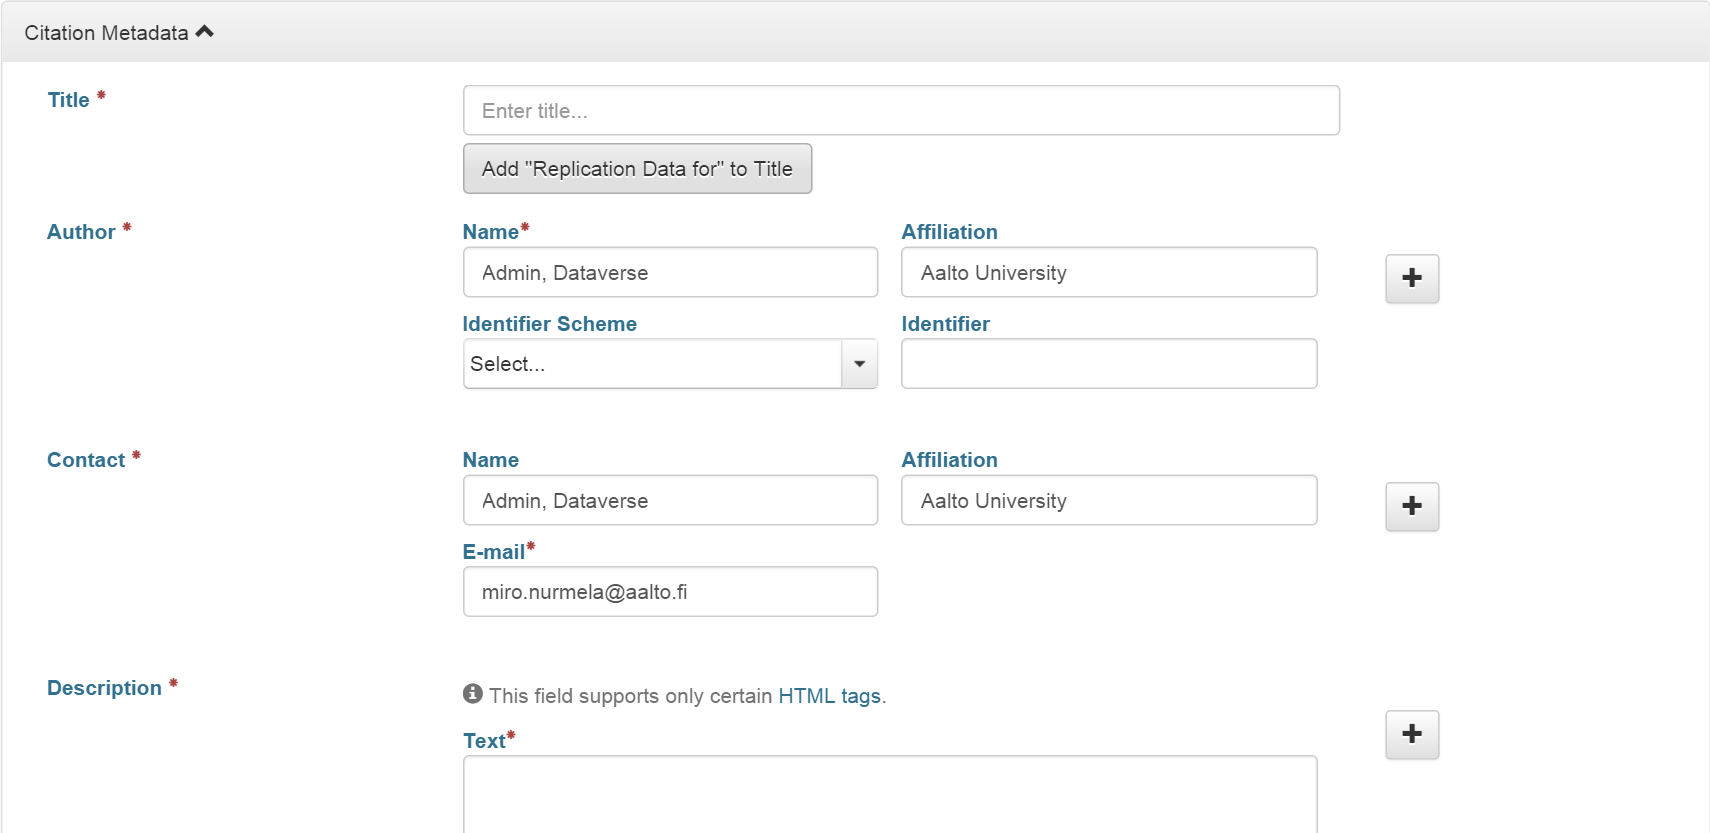
\includegraphics[width=\textwidth]{images/upload}
    \end{centering}
    \caption{A screen capture of the dataset upload form}
    \label{fig:upload}
\end{figure}

\begin{figure}
    \begin{centering}
        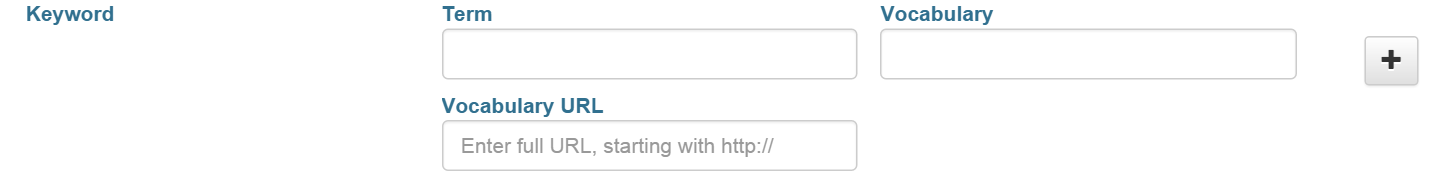
\includegraphics[width=\textwidth]{images/vocabulary}
    \end{centering}
    \caption{A screen capture of the confusion inducing vocabulary in the upload form}
    \label{fig:vocabulary}
\end{figure}

What is lacking of the upload process was the extended metadata that would be
important for the reuse of the data. The upload form contains the basic
metadata that is required to make the dataset searchable. Additional metadata,
such as details about the process of gathering the data, needs to be filled in
after the initial upload. The upload form contains a reminder, pictured in
Figure \ref{fig:hint}, to go add the metadata later. This approach has pros and
cons, since it makes the upload process easier but makes the metadata likely
lacking. Most users did not notice the hint to go add the metadata later and
those who did notice it did not know where the metadata addition would be done.

\begin{figure}
    \begin{centering}
        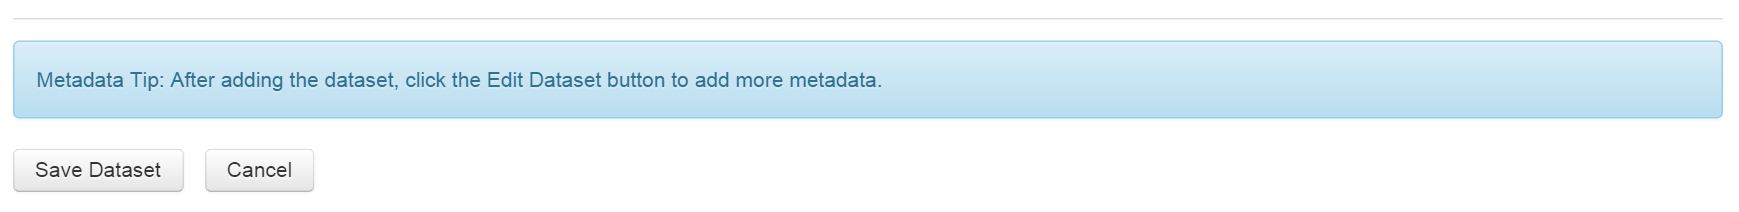
\includegraphics[width=\textwidth]{images/hint}
    \end{centering}
    \caption{A screen capture of the metadata reminder}
    \label{fig:hint}
\end{figure}

The search functionality is placed front and center in the user interface of
the Dataverse main page, as shown in Figure \ref{fig:search_main_page}. Users
easily locate the search bar and are able to start searching for relevant
datasets. The search results leave users lacking, however. This is not entirely
the fault of the search system, since the users found the names and short
descriptions of the datasets poor at describing the datasets which made
finding relevant datasets hard. Using the advanced search, which all the users
did not find, helps narrow down the options. The options in the
advanced search were noted to miss details. Details the users were missing
were dataset size and metadata related to their field. It was noted that
the system would work very well if you knew what you are looking for, for example
a scenario where your fellow researcher would have shared the identifier of
the dataset.

\begin{figure}
    \begin{centering}
        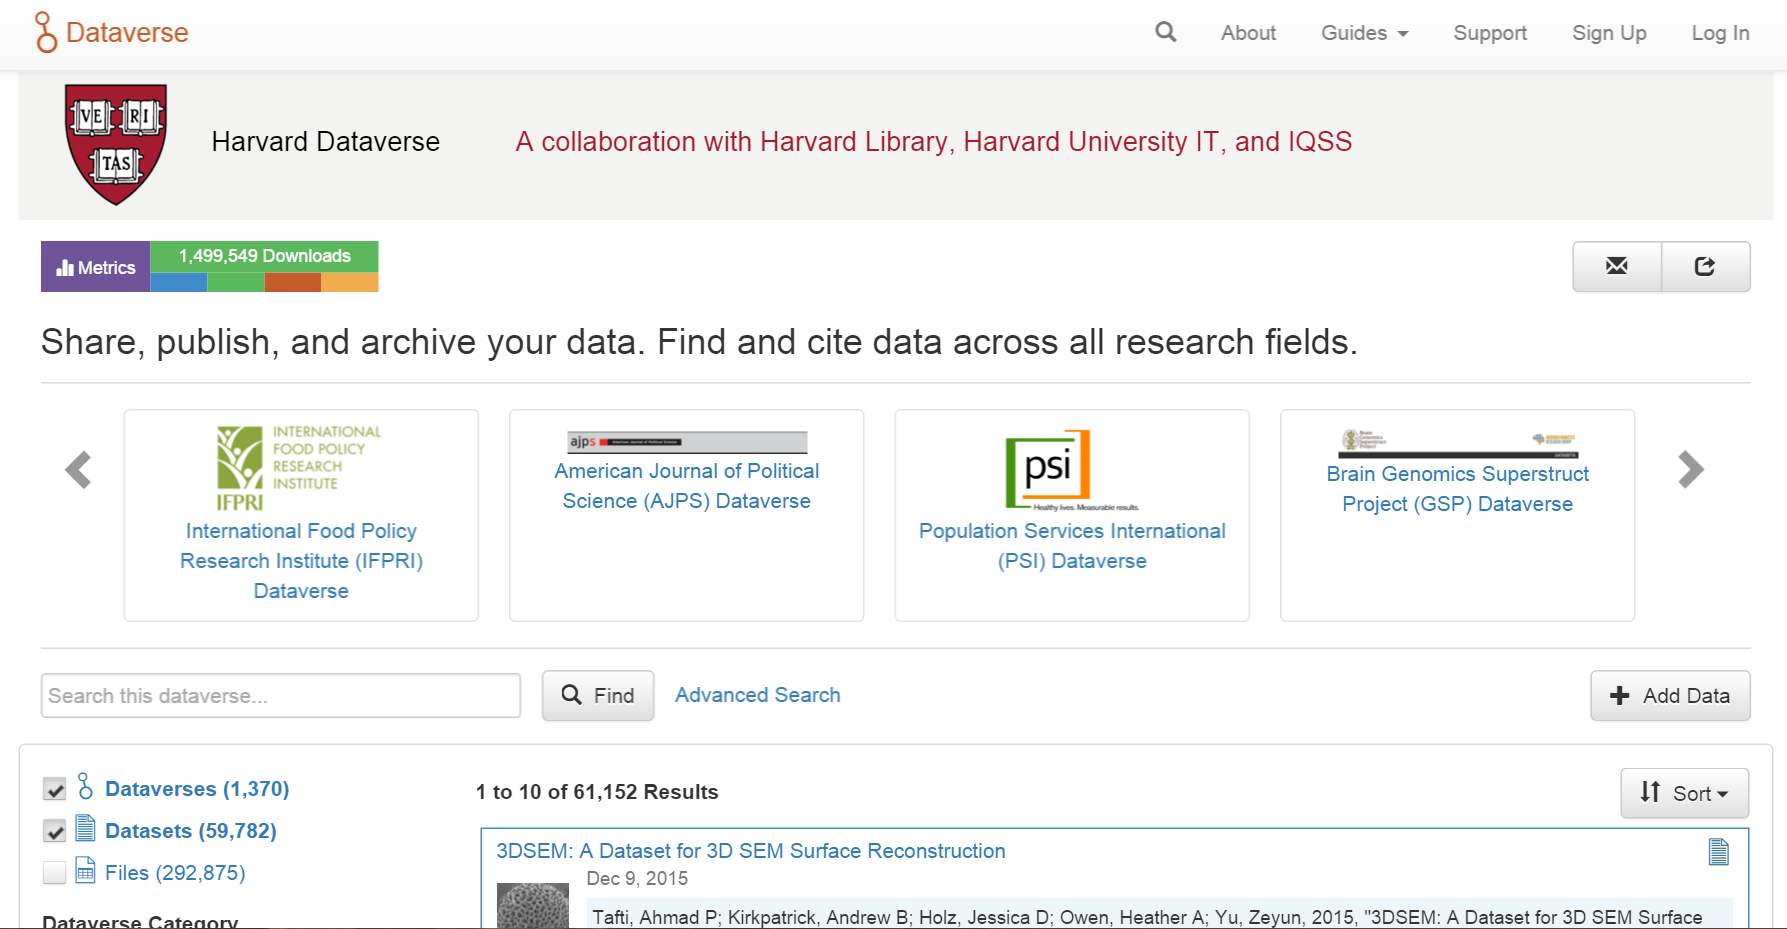
\includegraphics[width=\textwidth]{images/search_main_page}
    \end{centering}
    \caption{A screen capture of the Harvard Dataverse main page}
    \label{fig:search_main_page}
\end{figure}

The order in which the results are displayed is also unclear to the users.
The search results page offers the chance to sort the results, but that option
was missed by all users during the tests. The default setting is to sort the results by
relevance, but it is unclear to what relevance refers to in this context, since
the default search searches all searchable fields in datasets, Dataverses and files.
The fact that Dataverses, datasets and files are by default mixed in the search
results also does not help in finding relevant datasets. There is the option to
filter the files, datasets or Dataverses out of the search results, but the
option was fairly commonly missed by the users. It might be due to the novelty
of the terminology (Dataverse, especially, is a novel concept for the users).
An example of search results is shown in  Figure \ref{fig:search_results}.

\begin{figure}
    \begin{centering}
        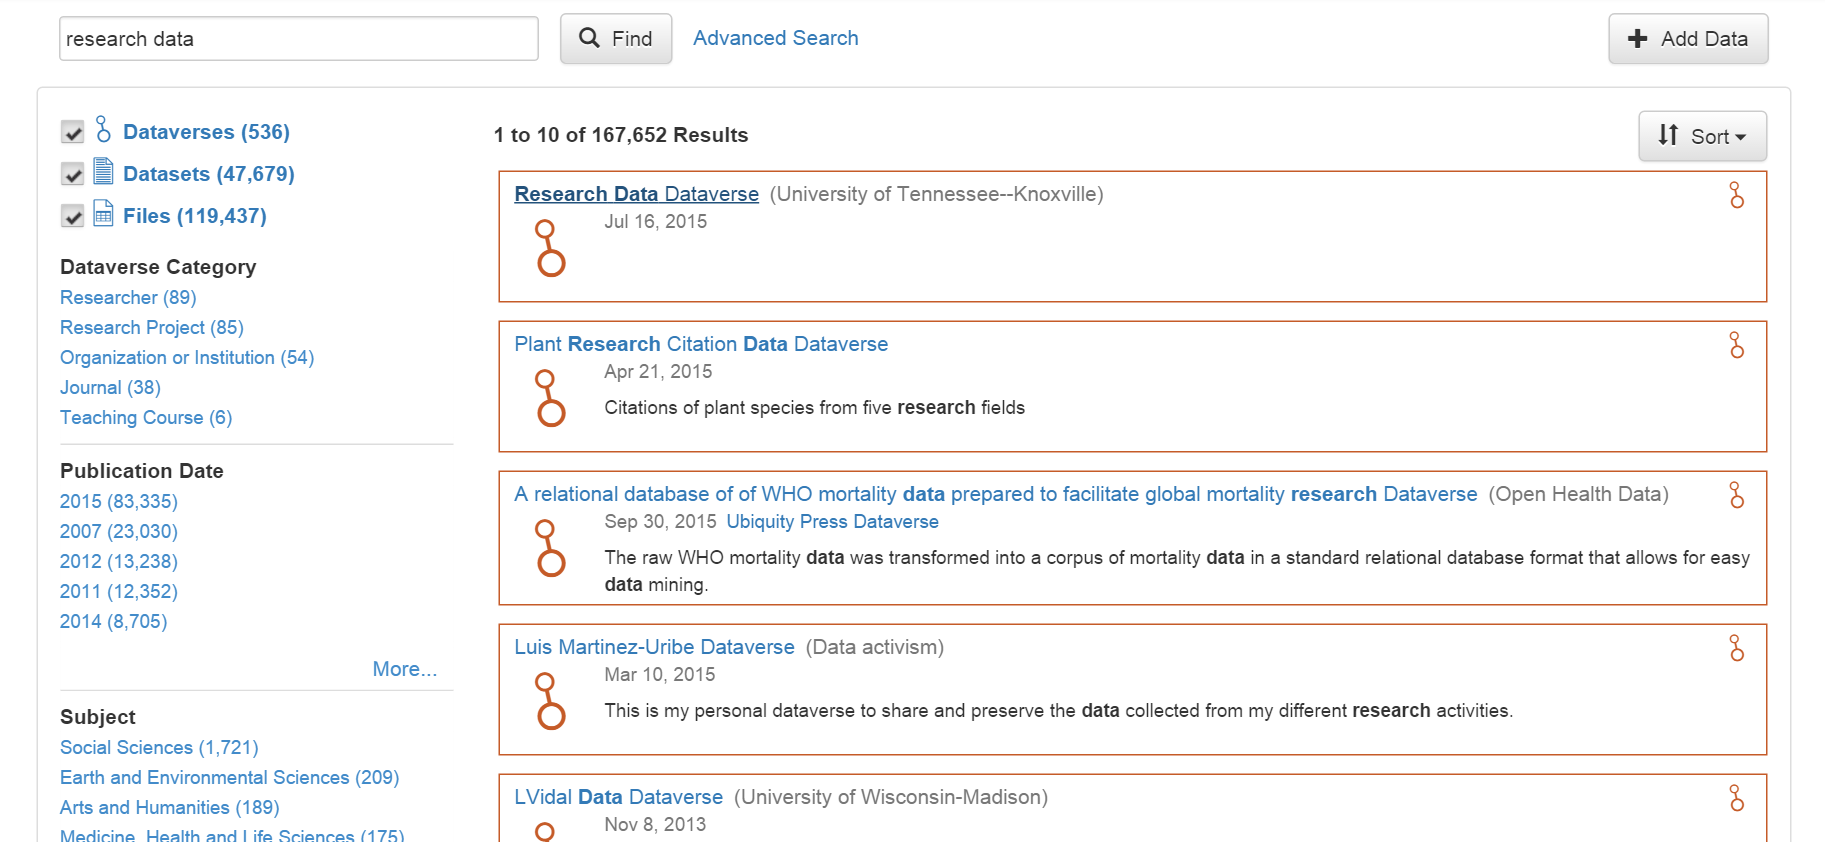
\includegraphics[width=\textwidth]{images/search_results}
    \end{centering}
    \caption{A screen capture of an example search results page}
    \label{fig:search_results}
\end{figure}

Dataverse implements helpful hover texts on the terms, as shown in Figure
\ref{fig:hovertext}. This feature went unnoticed by all users at first, but
most of them would find the feature by accident and find it helpful. It would
help if the helpful hover text would be indicated, for example, by a question
mark symbol next to the item to be explained.

\begin{figure}
    \begin{centering}
        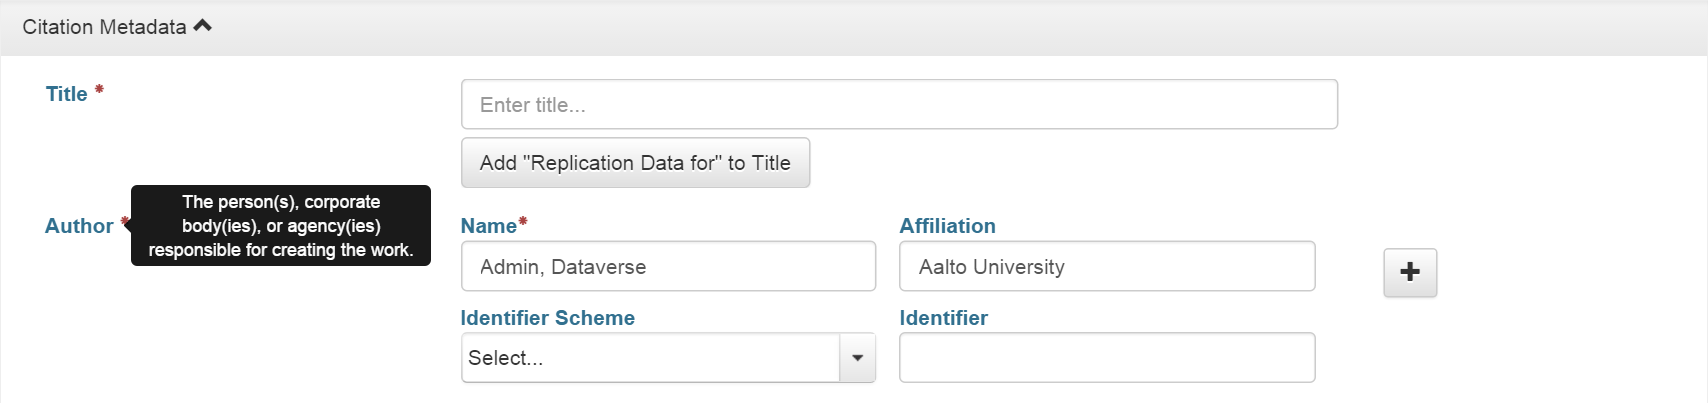
\includegraphics[width=\textwidth]{images/hovertext}
    \end{centering}
    \caption{A screen capture of the hover texts implemented in Dataverse}
    \label{fig:hovertext}
\end{figure}

What was common in both the contextual interviews and the lead user tests was
that the concept of publishing research data is novel for all the users. None
of them had published their research data online and few had used datasets from others,
but in those cases the datasets were always acquired by request and then
delivered using existing systems, such as Google Drive or email. When 
questioned on if they could make their research data public, for example with a tool
like Dataverse, many expressed that their research data had some privacy
concerns or other limitations to sharing or that it would take a considerable
amount of time to apply relevant metadata to make the datasets presentable.
Source code from some projects had been published in GitHub.

The contextual interviews and the lead user tests also shed light on the
current ways of managing research data. Network drives were used by the
users and their research groups to share all the data within the group, but
the there were no clear guidelines on how to describe dataset metadata or how
to organize the file structure on the network drives. This meant that it was
at times hard for the researchers to find relevant things from the drives and
for the new members of the groups to get acquainted with the system. It turned
out that currently research data management is not taught to the researchers,
but knowledge is gathered from peers and mistakes you make on your previous
projects.

The research data visualization, which came up as an interesting feature to
have in a research data publication platform during both the initial interviews
and the contextual interviews is implemented in Dataverse. The user feedback
on it, however, was that the visualization is very confusing and despite the
users being well versed in statistical methods could not understand what the
information displayed on the screen meant and how to get valuable information
out of it. Figure \ref{fig:tworavens} shows a view of the visualization tool.

\begin{figure}
    \begin{centering}
        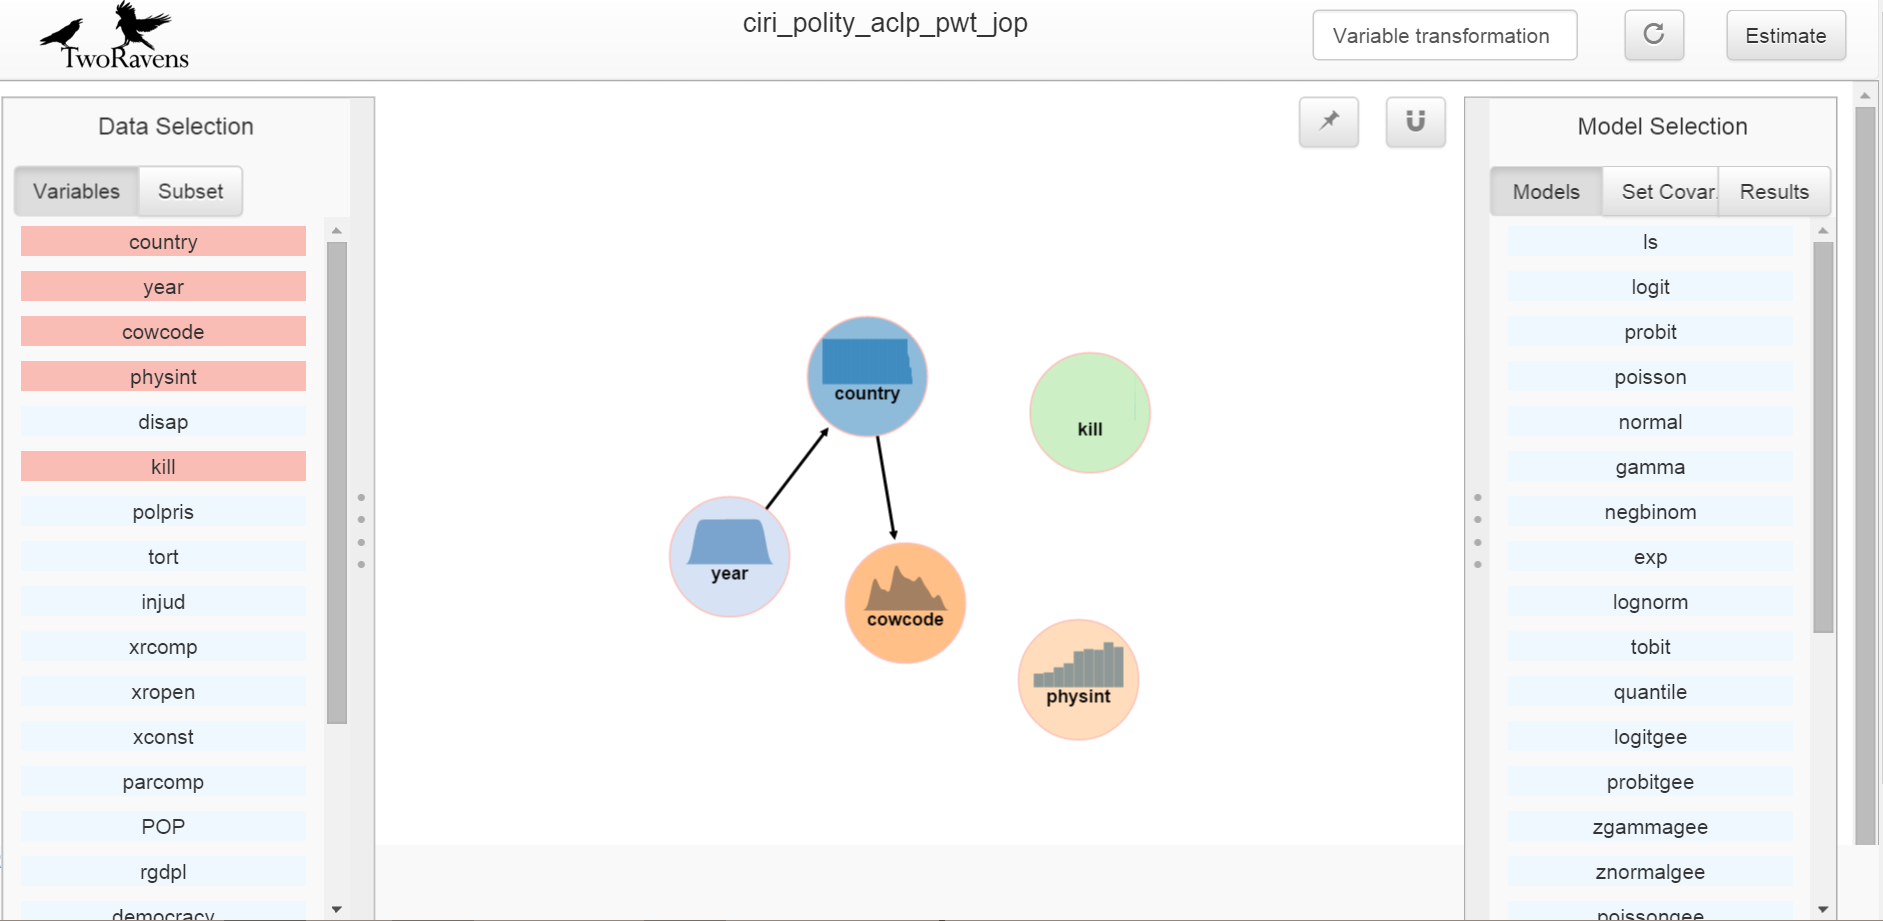
\includegraphics[width=\textwidth]{images/tworavens}
    \end{centering}
    \caption{A screen capture of Data visualization implemented in Dataverse}
    \label{fig:tworavens}
\end{figure}

The lead user tests mirrored the results from the contextual interviews when
it came down to the manual upload process of the datasets. Despite the lack of
previous knowledge on how to use the system or on how to publish research data
the lead users were able to learn the system and upload their datasets. After
working with the system for a longer time the need for computerized uploading
process became clear. For example, the user from the Sound Group had hundreds
of video files that could be uploaded to the publication system, but it would
not make sense to spend the time to do that manually. In addition some of that
data was being generated every day, so if that was to be published daily it
would require an automated system. The Dataverse offers a an API and a guide
for using it\footnote{\url{http://guides.dataverse.org/en/4.2/api/}}. The
user found that the guide with only example commands was
not enough to make the use of API easy. Coincidentally there is research
about research video data sharing which could be useful in the future when
video data needs to be shared~\cite{DBLP:conf/jcdl/SimonGSG15}.

After using the system for a longer time the users noted that the system could
help them access their datasets from outside the university's network. The
network drives and similar approaches in used nowadays limit the access to
the systems to the university network, which hinders both the ability of the
researchers to work on it from different computers as well as the ability to
share the information with collaborators from other places. There are, of
course, ways to access data within the university network with VPN or other
similar technologies, but that adds complexity to the process.

The longer period of use also brought up the fact that there is information in
how people store their data. For example, the folder structure of the network
drive might split files into subfolders by date of data collection. This serves
as implicit metadata, since there is no metadata file that tells that this
piece of data is from a certain date, but a human using the system would
understand it. Dataverse offers a chance to upload .zip file to the system
and this way preserving folder structures. In the case of
the Sound Group the video files are so large and there are so many of them
that uploading a huge file would make the reuse of that file very hard, not
to mention the uploading and downloading the file.

The installation and maintenance of the prototype Dataverse installation had
both flaws and good things to it. The basic installation following the
installation guide was easy, but adding in components like the TwoRavens or
Shibboleth authentication system was documented less clearly to the point that
it was not worth the effort to install the Shibboleth system for the prototype
solution. The TwoRavens installation process seemed to work, but the system
did not end up working in the prototype solution, so the TwoRavens was tested
with the actual Harvard Dataverse.

Codewise the Dataverse implementation is clean - it follows good object
oriented programming practices. Functionality is split into different
classes and the methods are short and well named. Dataverse has unit
tests implemented as well as a Jenkins
environment\footnote{\url{https://build.hmdc.harvard.edu:8443/}} for automated
integration tests. The test coverage is not very high - only
5\%\footnote{\url{https://coveralls.io/github/IQSS/dataverse}}.

User management with the Dataverse tools was easy. Dataverse offers a default
set of roles that cover the needs of research data publication process well.
Custom roles can also be made if the default ones are not enough.
Figure~\ref{fig:admin} shows the user management view of a single dataset. Permissions
can be changed for individual or groups, allowing the administrator of the
dataset to allow different parties to see the dataset before it is published.
Publishing will make it visible for all, but managing the permissions before
publishing the desired functionality of private publishing could be achieved.

\begin{figure}
    \begin{centering}
        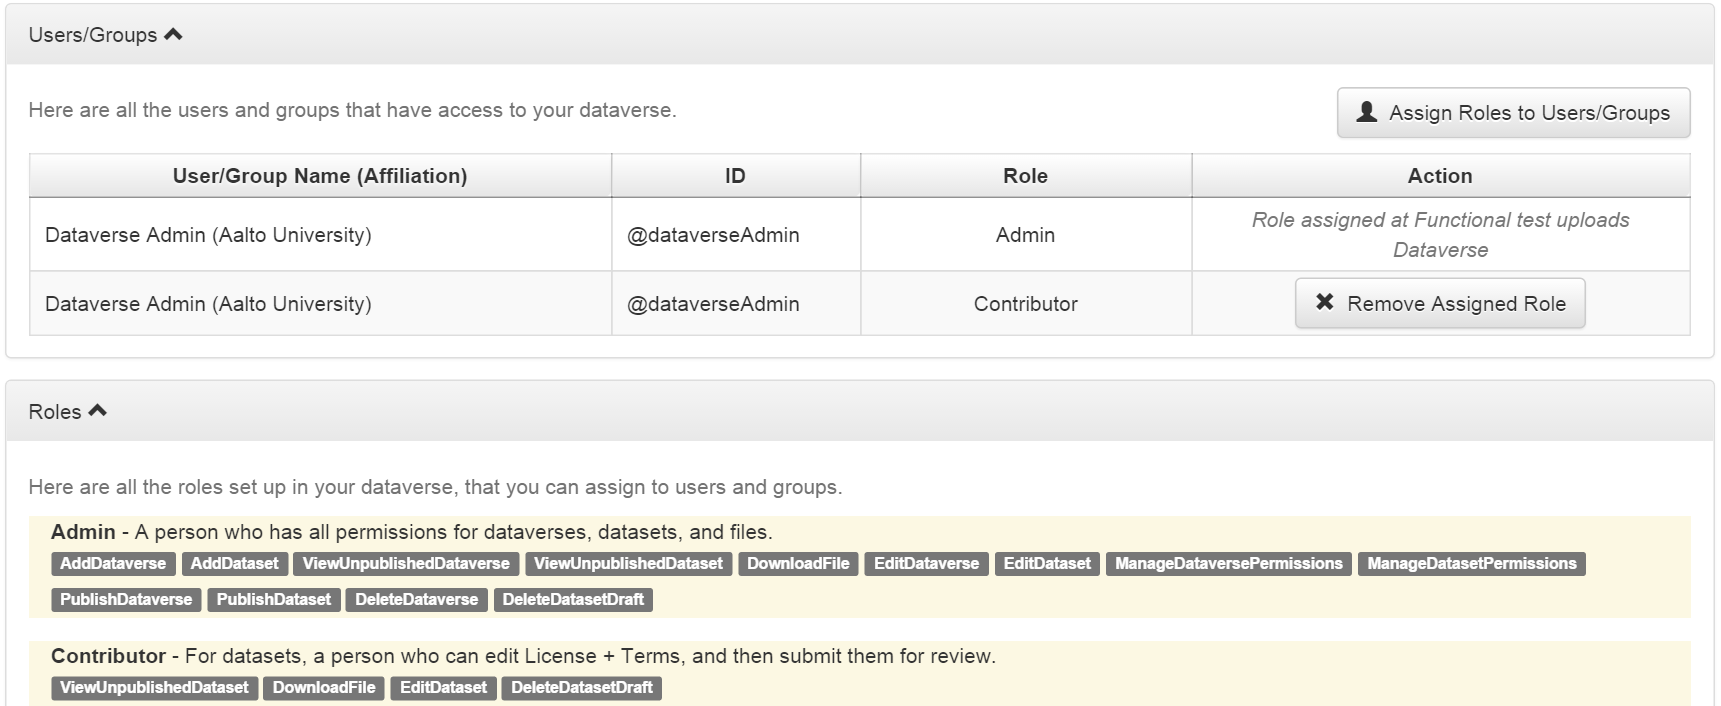
\includegraphics[width=\textwidth]{images/admin}
    \end{centering}
    \caption{A screen capture of the dataset user management view}
    \label{fig:admin}
\end{figure}

During the test on the development installation we came across an interesting
situation when the partition where the database of the Dataverse became too
full and no new datasets could be uploaded to the system. This did not crash
the system - the Dataverse could still be accessed and datasets be downloaded,
but new datasets could not be uploaded. Moving the database to a new partition
did not alone solve the problem since the failed dataset uploads had left
partial files to the Dataverse partition that prevented the Dataverse from
caching the new uploads. Once the fragmented remains of the failed uploads
were removed the and Dataverse had disk space to cache new datasets the system
started working again normally. It is good that the system was robust enough
to handle the insufficient space on the partition, but not cleaning up the
failed uploads caused frustration and the Dataverse documentation did not
help in resolving the issue.

Interesting note on Dataverse is that it gives DOIs to the published datasets.
This functionality is not documented, but digging into the code and the logs
from the system it turns out that that Dataverse uses the
EZID\footnote{\url{http://ezid.cdlib.org/}} service to supply DOIs for
datasets. What is strange is that when you set up your own Dataverse you
can just publish data and the DOIs will be given for you. This is strange
because registering DOIs is not free and it is hard to imagine that Harvard
would want to pay for all the DOIs for all the users of Dataverse.

In summary, Dataverse serves as a functional system to publishing research
data. The software is of good quality but the documentation and instructions
related to setting up the system could be better and the test coverage could be
improved. The mechanical processes of
uploading and searching datasets from the system work, but both of them could
be made more intuitive. Computerized upload of datasets is a must have feature
when dealing with datasets that contain a large amount of files. In addition to
taking care of these technical matters, training for research data management
and integration of research data publishing to the workflow of scientists is
required.

\iffalse
\begin{itemize}
    \item The manual uploading process is just fine
    \item It is a must that there is an API - for example, thousands of video
          files will not be uploaded manually
    \item It is important that the server can cache large files as a part of
          the upload process
    \item Search functionality
        \begin{itemize}
            \item Poorly described datasets
            \item Not intuitive to find data from within all the search results
            \item Dataset size is no available as a search filtering parameter
            \item The vocabulary in advanced search is foreign for the users
            \item The search results are not well organized
        \end{itemize}
    \item Access controls are important and function quite well
    \item Peer to peer teaching would be good
    \item How data is stored (folder structures and such) contains information
          and that should be captured by the system
    \item Accessing data from outside work computers would be nice
    \item More to come here, have to dig up my notes
\end{itemize}
\fi
